% -*- coding: UTF-8 -*-
\documentclass{article}
\usepackage{amsmath}
\usepackage{tikz}

\begin{document}
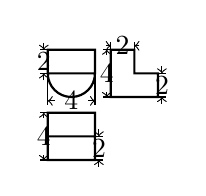
\begin{tikzpicture}

  \draw[thick] (-0.1,0.7) rectangle (-0.7,0.4)
               (-0.7,0.4) arc (-180:0:0.3)
               (0.1,0.1) -- (0.7,0.1) -- (0.7,0.4) -- (0.4,0.4) -- (0.4,0.7) -- (0.1,0.7) -- cycle
               (-0.7,-0.1) rectangle (-0.1,-0.4) rectangle (-0.7,-0.7);
  \draw (-0.7,0.7) -- (-0.8,0.7) (-0.7,0.4) -- (-0.8,0.4) (-0.7,0.4) -- (-0.7,0) (-0.1,0.4) -- (-0.1,0) (0.1,0.7) -- (0,0.7) (0.1,0.1) -- (0,0.1) (0.1,0.7) -- (0.1,0.8) (0.4,0.7) -- (0.4,0.8) (0.7,0.1) -- (0.8,0.1) (0.7,0.4) -- (0.8,0.4) (-0.7,-0.1) -- (-0.8,-0.1) (-0.7,-0.7) -- (-0.8,-0.7) (-0.1,-0.4) -- (0,-0.4) (-0.1,-0.7) -- (0,-0.7);

  \node (n) at (-0.75,0.55) {$2$};
  \node (n0) at (-0.4,0.05) {$4$};
  \node (n1) at (0.25,0.75) {$2$};
  \node (n2) at (0.05,0.4) {$4$};
  \node (n3) at (0.75,0.25) {$2$};
  \node (n4) at (-0.75,-0.4) {$4$};
  \node (n5) at (-0.05,-0.55) {$2$};

  \draw[->] (n) -- (-0.75,0.7);
  \draw[->] (n) -- (-0.75,0.4);
  \draw[->] (n0) -- (-0.7,0.05);
  \draw[->] (n0) -- (-0.1,0.05);
  \draw[->] (n1) -- (0.1,0.75);
  \draw[->] (n1) -- (0.4,0.75);
  \draw[->] (n2) -- (0.05,0.7);
  \draw[->] (n2) -- (0.05,0.1);
  \draw[->] (n3) -- (0.75,0.1);
  \draw[->] (n3) -- (0.75,0.4);
  \draw[->] (n4) -- (-0.75,-0.7);
  \draw[->] (n4) -- (-0.75,-0.1);
  \draw[->] (n5) -- (-0.05,-0.4);
  \draw[->] (n5) -- (-0.05,-0.7);

\end{tikzpicture}
\end{document}
